\documentclass[tikz]{standalone}

\usepackage{tikz}
\usetikzlibrary{decorations.markings}
\usetikzlibrary{arrows.meta}
\usetikzlibrary{calc}

\usepackage{amsmath}

\begin{document}


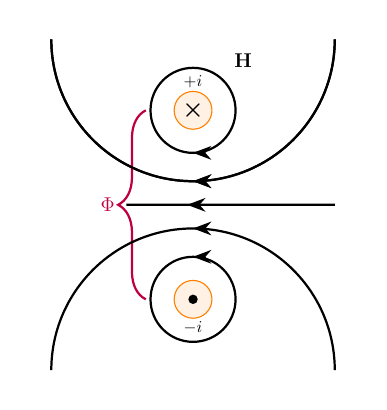
\begin{tikzpicture}[scale=0.6, transform shape]

% Define styles
\tikzset{
    charge/.style={fill=orange!10, draw=orange, circle, radius=0.4},
    fieldline/.style={thick, postaction={decorate}, decoration={markings}},
    arrow/.style={decoration={mark=at position #1 with {\arrow{Stealth}}}},
    reversearrow/.style={decoration={mark=at position #1 with {\arrowreversed{Stealth}}}}
}

% grind lines
%\draw[help lines, dashed] grid (10,10);

% zeige den Teil, der durch die Graphik benutzt wird
\useasboundingbox (1.5,1.25) rectangle (8.5,8.75);


%position of bottom wire
\coordinate (A1) at (5,3);

%position of top wire
\coordinate (A2) at (5,7);

% Negative charge node
\draw[charge] (A1) circle node[below=0.2cm] {$-i$};
\node[circle, fill=black, inner sep=2pt] at (A1) {};

% Positive charge node
\draw[charge] (A2) circle node[above=0.2cm] {$+i$};
\node at (A2) {\Large$\boldsymbol{\times}$};

% Magnetic field lines
\draw[fieldline, reversearrow=0.5] (2,8.5) arc (-180:0:3cm and 3cm);

% magnetic flux
\draw [thick, purple, decorate, decoration={brace, amplitude=10pt}] ($(A1) + (-1cm, 0)$) -- ($(A2) + (-1cm, 0)$)
node[midway, left=15pt] (FLUX) {\large $\Phi$};

% Magnetic field lines
\draw[fieldline, reversearrow=0.5] (2,8.5) arc (-180:0:3cm and 3cm);
\draw[fieldline, reversearrow=0.75] (5,7) circle[radius=0.9];
\draw[fieldline, arrow=0.69, shorten >=2pt] (8,5) -- (FLUX);
\draw[fieldline, reversearrow=0.5] (2,1.5) arc (180:0:3cm and 3cm);
\draw[fieldline, arrow=0.25] (5,3) circle[radius=0.9];


% Magnetic field label
\node at ($(A2)+(45:1.5)$) {\large \textbf{H}};

\end{tikzpicture}


\end{document}